\documentclass[sigconf,nonacm]{acmart}
\settopmatter{printacmref=false,printfolios=true,authorsperrow=1}
\setcopyright{none}
\renewcommand\footnotetextcopyrightpermission[1]{}
\usepackage{amsmath,booktabs,tabularx,array,enumitem,balance,graphicx,xcolor,seqsplit}
\definecolor{CourseBlue}{HTML}{315EFB}
\definecolor{CourseTeal}{HTML}{14877D}
\definecolor{CourseInk}{HTML}{18324A}
\hypersetup{colorlinks=true,linkcolor=CourseBlue,citecolor=CourseTeal,urlcolor=CourseTeal}
\newcolumntype{Y}{>{\raggedright\arraybackslash}X}
\setlist{leftmargin=*,topsep=2pt,itemsep=1pt}
\newcommand{\CourseNumber}{COMSCI/ECON 206}
\newcommand{\CourseName}{Computational Microeconomics}
\newcommand{\CourseSession}{Autumn 2026 Session 1}
\newcommand{\Instructor}{Professor Luyao Zhang}
\newcommand{\TeamCode}{FP10}
\newcommand{\SymposiumSession}{Not yet assigned}
\newcommand{\ComputationalCommit}{\texttt{\seqsplit{791e12224576e5963fd5672f8f90acdcea5556a0}}}
\newcommand{\BehavioralCommit}{\texttt{\seqsplit{ea7ce241de34b8d21b036d39157ca974c019bb31}}}
\newcommand{\StaticCommit}{\texttt{\seqsplit{a9c51af0b685003f770cce47d810607823847353}}}
\newcommand{\SpaceRepo}{\href{https://huggingface.co/spaces/dku-comsci-econ206-2026/ps2-share-or-hide-drone-disclosure}{Hugging Face Space repository}}
\newcommand{\DirectApp}{\href{https://dku-comsci-econ206-2026-ps2-share-or-hide-drone-96834c7.static.hf.space/index.html}{direct static app}}
\newcommand{\coursemeta}{\noindent\textbf{Submission to:} \CourseNumber{} -- \CourseName.\\
\textbf{Course session:} \CourseSession. \textbf{Team:} \TeamCode. \textbf{Symposium:} \SymposiumSession.\\
\textbf{Course instructor:} \Instructor. \textbf{Assignment:} PS2 collaborative research proposal.\par}

\title{Share or Hide? Strategic Disclosure in Congested Low-Altitude Drone Traffic}
\author{Yiqiao Liu}
\affiliation{\institution{Duke Kunshan University}\city{Kunshan}\country{China}}
\renewcommand{\shortauthors}{Liu (Team FP10)}

\begin{document}
\maketitle
\raggedbottom
\coursemeta
\balance

\section{Shared Question and Verified Gap}
Competing drone operators can coordinate better when they share flight intent, but precise routes and timing can reveal demand patterns to rivals. Existing AAM studies design centralized full-information systems, decentralized limited-information protocols, or privacy-preserving allocation mechanisms \cite{chin2022efficient,chin2023traffic,maheshwari2025privacy}. The unresolved design choice is not whether privacy matters, but how much commercially sensitive detail a strategic operator voluntarily releases. We ask: \emph{when confidentiality costs are private, how does voluntary disclosure change with congestion, when does equilibrium differ from the full-information first best, and can a congestion-contingent access rule narrow that gap?} Residual corridor scarcity is allocated downstream, rather than treated as the central contribution.

The defensible distinction is narrow: prior AAM work largely specifies the sharing protocol as part of system design, whereas this project makes disclosure granularity an endogenous action with privately known commercial-confidentiality costs and congestion-dependent coordination value. This connects AAM privacy design to economic work on incentives to share private information among competitors \cite{raith1996general} without claiming priority over either literature.

\section{Strategic Model and Three Lenses}
The core is a static Bayesian game with incomplete information. Operators $N=\{A,B\}$ simultaneously choose $a_i\in\{M,P,F\}$: Minimum, Partial, or Full \emph{voluntary commercial} disclosure. Minimum never withholds legally required or safety-critical information. Each privately observes $c_i\in\{c_L,c_H\}=\{1,1.6\}$, independently with $\Pr(c_i=c_L)=0.5$; public congestion is $d\in\{0.3,0.6,1\}$. Let $x(M,P,F)=(0,1,2)$ and $k(M,P,F)=(0,1,2.5)$. The normalized payoff is
\begin{equation}
u_i(a_i,a_j;c_i,d)=dB[1-e^{-\lambda(x_i+x_j)}]-c_i k(a_i),
\end{equation}
where $B=7.5$ and $\lambda=0.5$. These are stylized benchmark quantities, not empirical dollar estimates. Exhaustive enumeration of all $9\times9=81$ pure Bayesian strategy profiles yields a unique pure-strategy BNE at each benchmark congestion: by type order $(L,H)$, Low is $(M,M)$, Medium is $(P,M)$, and High is $(P,P)$. Thus disclosure rises with congestion, with an intermediate region in which only the low-cost type shares more. Full is absent because coordination benefits diminish while Full has a relatively steep exposure cost; this is an economic implication of the benchmark, not a solver failure.

The social-choice lens defines $W=u_A+u_B$ and compares equilibrium to a planner who observes realized types. Expected BNE/first-best welfare (gap $W_{FB}-W_{BNE}$) is Low $0.000/0.639$ ($0.639$), Medium $2.193/3.139$ ($0.946$), and High $6.882/7.385$ ($0.503$). The largest benchmark loss therefore occurs at intermediate, not maximum, congestion: at High even the confidentiality-sensitive type chooses Partial, while at Medium socially useful sharing remains privately unattractive to that type. Some first-best profiles are asymmetric -- $(M,P)$ and $(P,M)$ tie for Low $H/H$, while $(P,F)$ and $(F,P)$ tie for High $L/L$ -- so efficiency can concentrate disclosure burden even without a formal distributive-welfare model.

\begin{figure*}[t]
  \centering
  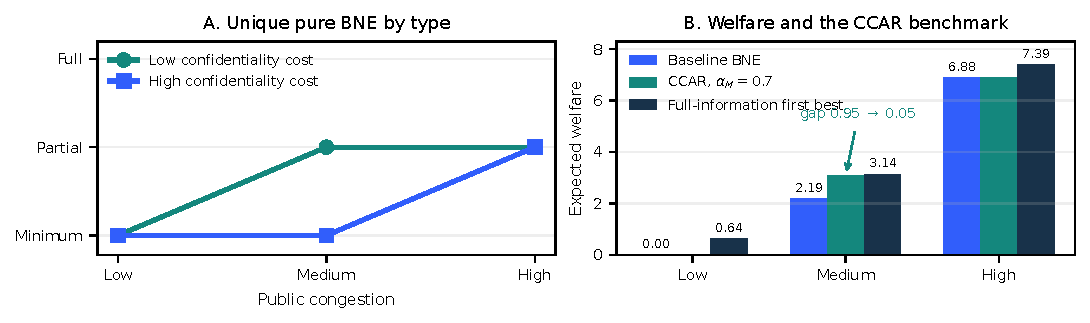
\includegraphics[width=\textwidth]{figures/main_results.pdf}
  \caption{Validated benchmark results generated from tracked CSV outputs. Panel A reports each operator's type-contingent action in the unique pure BNE. Panel B compares underlying expected welfare; at Medium, CCAR changes the BNE from $(P,M)$ to $(P,P)$ by type and reduces the gap from $0.946$ to $0.050$. The Low and High CCAR bars coincide with the baseline.}
  \Description{Two panels show increasing equilibrium disclosure with congestion and grouped welfare bars for baseline BNE, CCAR, and the full-information first best.}
  \label{fig:main-results}
\end{figure*}

\section{Computation, Mechanism, and Allocation}
The computational lens directly evaluates utilities, enumerates all pure BNE without imposing symmetry, preserves first-best ties, and separates mechanism utility from underlying welfare. Figure~\ref{fig:main-results} is generated only from validated CSVs. For the candidate Congestion-Contingent Access Rule (CCAR), mandatory safety information remains unconditional; only enhanced non-safety services -- higher-resolution forecasts, rerouting information, and richer aggregate predictions -- depend on voluntary disclosure. At Low, $\alpha(M)=\alpha(P)=\alpha(F)=1$. At Medium/High, $\alpha(P)=\alpha(F)=1$ and $\alpha(M)=\alpha_M$, so $u_i^{CCAR}=\alpha(a_i,d)dB[1-e^{-\lambda(x_i+x_j)}]-c_i k(a_i)$. With $\alpha_M=0.7$, Medium changes from $(P,M)$ to $(P,P)$ and underlying welfare rises $2.193\rightarrow3.089$, moving the gap $0.946\rightarrow0.050$. This is a benchmark result, not proof of universal superiority.

Indeed, a 760-cell $(c_H,\alpha_M,d)$ search finds 401 cells with no equilibrium-set effect, 334 with the stated robust welfare improvement diagnostic, 18 with excessive disclosure, 3 with a larger gap than the worst baseline gap, 66 with multiple pure BNE, and 0 with no pure BNE; categories overlap and are neither frequencies nor probabilities. Grid transitions are approximate. At Medium, the $\alpha_M$ sweep gives $(P,P)$ through $0.70$, two asymmetric equilibria at $0.75$, and the baseline $(P,M)$ from $0.80$ onward.

The Week 5 application allocates one priority slot in a congested corridor among eligible non-emergency commercial operators; emergency/public-safety flights stay outside payment. With values $(8,5,3,2)$ and FCFS order $(B,C,A,D)$, FCFS awards $B$ the slot (efficiency $5/8=0.625$). A truthful sealed-bid second-price auction awards $A$, charges $5$, and gives winner utility $3$ and efficiency $1$ \cite{vickrey1961counterspeculation}. In 10,000 seeded IPV rounds with four $U[0,10]$ bidders, mean FCFS efficiency is $0.622308$ versus $1.000000$ for truthful second price. Payments are transfers in welfare. Ability to pay, social urgency, unequal access, common/interdependent values, and monetization concerns prevent a blanket policy ranking; related AAM work also treats auctions as one component of coordination \cite{chin2023traffic,su2024vertiport}.

\section{Behavior and Interdisciplinary Integration}
The working behavioral artifact elicits a Solo Decision with a hidden rival type, an $M/P/F$ choice and motivation, then reveals the model benchmark; a second round introduces CCAR. Same-device Peer Play supports paired discussion, and an optional auction module links downstream scarcity. Reset/isolation and an explicit evidence boundary are built in. No accounts, PII, external LLM calls, or durable telemetry are used. The artifact is a decision probe, \emph{not representative behavioral data}: it can discriminate whether choices respond to congestion, confidentiality type, or reciprocal access, but the current paper makes no participant-level claim.

Artifacts: \SpaceRepo; \DirectApp. The validated computational checkpoint is identified in Appendix~\ref{app:repro}. No GitHub remote or public runnable-notebook URL is configured; this is recorded rather than replaced by an invented link.

\section{Contribution, Leadership, and Roadmap}
The project integrates three lenses: Bayesian incentives identify voluntary disclosure; computation verifies equilibrium, welfare, and failure regions; behavioral design exposes assumptions to choice and reflection. Its practical contribution is a testable governance proposition: enhanced non-safety coordination access may encourage useful sharing at intermediate congestion, but only with explicit safeguards for mandatory safety, privacy, fairness, and parameter sensitivity. Next steps are empirical calibration, mixed and repeated equilibria, correlated types, enforcement and administrative costs, and classroom or field data collected under a reviewed protocol. Team FP10 is a single-author team; intellectual ownership, validation, and final submission responsibility remain with Yiqiao Liu. The A0 poster and symposium-session assignment remain pending course logistics.

\clearpage
\section*{Author Notes}
\textbf{Joint authorship and named contribution.} Team FP10 has one member, Yiqiao Liu. Liu formulated the research question, selected the disclosure actions and welfare comparison, interpreted CCAR as access to enhanced non-safety services, bounded the auction extension, specified the behavioral decision flow, reviewed the implementation, and accepts responsibility for every claim. The computational implementation, debugging, sensitivity analysis, static deployment, literature-search support, formatting, and drafting/editing were assisted by AI tools. Numerical results were generated and validated by reproducible code rather than accepted from generated prose. No additional team member or uncredited collaborator is represented.

\textbf{Course-artifact status.} The source repository currently has no remote; the exact local commits are recorded in Appendix~\ref{app:repro}. The public behavioral Space is live. The A0 poster has not been supplied in this package, and the symposium session has not yet been assigned.

\bibliographystyle{ACM-Reference-Format}
\bibliography{references}

\appendix
\section{Model Specification}
\label{app:model}
Nature independently draws $c_A,c_B\in\{1,1.6\}$ with equal probability and publicly reveals $d$. Each operator observes its own type, not its rival's, then simultaneously chooses $M,P,$ or $F$. Payoffs follow Equation~(1). A pure strategy is a map $s_i:\{L,H\}\rightarrow\{M,P,F\}$, written in $(L,H)$ order. The solution concept is pure-strategy Bayesian Nash equilibrium: every type's prescribed action maximizes interim expected utility against the rival's type-contingent strategy. The code enumerates all nine strategies per operator and all 81 strategy profiles. Safety-critical and legally required information lies outside the action set.

\begin{table}[H]
\caption{Normalized benchmark primitives.}
\centering
\small
\begin{tabular}{@{}ll@{}}
\toprule
Primitive & Value \\
\midrule
Actions $(M,P,F)$ & $x=(0,1,2)$; $k=(0,1,2.5)$ \\
Types $(L,H)$ & $c=(1,1.6)$; prior $(0.5,0.5)$ \\
Congestion $(L,M,H)$ & $d=(0.3,0.6,1.0)$ \\
Coordination technology & $B=7.5$, $\lambda=0.5$ \\
\bottomrule
\end{tabular}
\end{table}

\section{Baseline Equilibrium Verification}
\label{app:bne}
For each own type $t$ and rival strategy $s_j$, the verifier computes
\[
EU_i(a\mid t,s_j,d)=\sum_{t_j\in\{L,H\}}\Pr(t_j)u_i(a,s_j(t_j);t,d).
\]
Table~\ref{tab:eu} reports all deviations against the equilibrium rival strategy; bold values are maximizing actions. The same calculation is applied to both operators, and no symmetry restriction is imposed.

\begin{table*}[t]
\caption{Interim expected utility of each action against the benchmark equilibrium rival strategy. The rival strategy and chosen action are ordered by own type $(L,H)$.}
\label{tab:eu}
\centering
\small
\begin{tabular}{@{}llcrrrl@{}}
\toprule
Congestion & Own type & Rival strategy & $EU(M)$ & $EU(P)$ & $EU(F)$ & Equilibrium choice \\
\midrule
Low & $L$ & $(M,M)$ & \textbf{0.000} & -0.115 & -1.078 & $M$ \\
Low & $H$ & $(M,M)$ & \textbf{0.000} & -0.715 & -2.578 & $M$ \\
Medium & $L$ & $(P,M)$ & 0.885 & \textbf{1.308} & 0.670 & $P$ \\
Medium & $H$ & $(P,M)$ & \textbf{0.885} & 0.708 & -0.830 & $M$ \\
High & $L$ & $(P,P)$ & 2.951 & \textbf{3.741} & 3.327 & $P$ \\
High & $H$ & $(P,P)$ & 2.951 & \textbf{3.141} & 1.827 & $P$ \\
\bottomrule
\end{tabular}
\end{table*}


\section{Social-Welfare Calculation}
\label{app:welfare}
Baseline welfare is the transfer-free sum $W=u_A+u_B$. For each realized $(c_A,c_B,d)$, the full-information first best exhaustively maximizes $W$ over the nine action profiles and preserves ties; expectation then uses the independent prior. This benchmark assumes type observability and need not be implementable. Table~\ref{tab:firstbest} makes the realized-type comparison auditable.

\begin{table*}[t]
\caption{Full-information first-best action profiles and welfare by realized types.}
\label{tab:firstbest}
\centering
\small
\begin{tabular}{@{}llrrr@{}}
\toprule
Congestion & Type pair & Maximizing profile(s) & Tie count & Welfare \\
\midrule
Low & $L/L$ & $(P,P)$ & 1 & 0.845 \\
Low & $L/H$; $H/L$ & $(P,M)$; $(M,P)$ & 1 each & 0.771 \\
Low & $H/H$ & $(M,P)$; $(P,M)$ & 2 & 0.171 \\
Medium & $L/L$ & $(P,P)$ & 1 & 3.689 \\
Medium & $L/H$; $H/L$ & $(F,M)$; $(M,F)$ & 1 each & 3.189 \\
Medium & $H/H$ & $(P,P)$ & 1 & 2.489 \\
High & $L/L$ & $(P,F)$; $(F,P)$ & 2 & 8.153 \\
High & $L/H$; $H/L$ & $(F,P)$; $(P,F)$ & 1 each & 7.553 \\
High & $H/H$ & $(P,P)$ & 1 & 6.282 \\
\bottomrule
\end{tabular}
\end{table*}

\section{CCAR Mechanism}
\label{app:ccar}
CCAR scales only an operator's access to enhanced, non-safety coordination value. It never conditions mandatory safety information. At Low congestion all access factors equal one. At Medium and High, $M$ receives $\alpha_M$ and $P,F$ receive one. Equilibrium uses CCAR operator utility, but reported ``underlying welfare'' removes the artificial access penalty before summing utilities; this prevents restricted service access from being counted as a social benefit. At $\alpha_M=0.7$, Medium has unique $(P,P)$ strategies for both operators, underlying welfare $3.089$, operator-utility sum $3.089$, and first-best welfare $3.139$. Low remains $(M,M)$; High remains $(P,P)$. The mechanism is a candidate design, not an optimality theorem.

\section{Sensitivity Analysis}
\label{app:sensitivity}
The tracked analysis varies $\alpha_M$, the high confidentiality coefficient $c_H$, and the Full exposure multiplier $k(F)$. The $\alpha_M$ benchmark grid shows a discontinuous equilibrium-set change around the reported grid cells; it does not establish an analytical cutoff. Lowering $k(F)$ can make Full a best response or an equilibrium action, confirming that its benchmark absence is driven by diminishing coordination gains relative to exposure cost. The 760-cell failure search reports overlapping diagnostics: 401 no-effect, 334 robust-improvement, 18 excessive-disclosure, 3 increased-gap, 66 multiple-BNE, and 0 no-pure-BNE cells. These are design-grid counts, not empirical frequencies. Multiple equilibria require a selection rule before policy prediction.

\section{Auction Laboratory Record}
\label{app:auction}
\begin{description}[style=nextline]
\item[Resource and participants.] One priority-access slot in a congested low-altitude corridor for a fixed short window; eligible non-emergency commercial operators only.
\item[Information and reports.] In the benchmark, four bidders have iid private values $U[0,10]$ and submit sealed bids. The deterministic example uses values $A=8,B=5,C=3,D=2$; FCFS order is $B,C,A,D$.
\item[Rules.] FCFS stops at the first eligible request. The single-unit second-price auction allocates to the highest bid, breaks ties by operator ID, and charges the second-highest bid.
\item[Rational benchmark.] With independent private values, truthful bidding is weakly dominant in the Vickrey auction \cite{vickrey1961counterspeculation}. Payments are transfers; modeled social welfare equals allocated value.
\item[Computed comparison.] The example produces FCFS efficiency $0.625$ and truthful-auction efficiency $1$. Across 10,000 rounds (seed 206), means are $0.622308$ and $1.000000$; mean allocated values are $4.96856$ and $7.99983$, and mean second-price revenue is $5.99207$.
\item[Stress test and boundary.] With mean-one lognormal bid noise (seed 1206), efficiency is 0.989514 and misallocation is 0.1393 at $\sigma=0.1$; the corresponding values are 0.956564 and 0.2783 at $0.25$, 0.904572 and 0.4124 at $0.5$, and 0.826281 and 0.5467 at $1.0$. This is a bounded-rationality perturbation, not equilibrium behavior. Common values, urgency, wealth, and institutional legitimacy are omitted.
\end{description}

\section{Behavioral Artifact}
\label{app:behavior}
The Solo flow assigns a participant a confidentiality type and congestion state, hides the rival type, records an $M/P/F$ choice plus a motivation/reflection prompt, and reveals the computational benchmark only after choice. A CCAR round then tests whether reciprocal access changes the decision. Peer Play lets two people use one device; the optional auction demonstrates the bounded allocation extension. Model Results and About/Methods expose assumptions and the evidence boundary. Reset and session isolation were browser-tested. The static deployment loads provenance-tagged JSON exported from the validated Python model and performs finite lookups plus auction arithmetic locally. It collects no PII, creates no accounts, calls no external LLM, and stores no durable telemetry. It is a working decision artifact, not a behavioral dataset.

\section{Reproducibility}
\label{app:repro}
\noindent\textbf{Validated commits.}\par
\noindent Computational: \ComputationalCommit\\
Behavioral: \BehavioralCommit\\
Static deployed artifact: \StaticCommit\par
The verified suite contains 27 computational, 17 Gradio behavioral, and 15 static/export tests: 59 total, 0 failed. The project recommends Python 3.13; recorded runs used Python 3.13.7 with NumPy 2.3.5 and Matplotlib 3.10.8. The notebooks are \texttt{\seqsplit{01\_strategic\_disclosure\_game.ipynb}} and \texttt{\seqsplit{02\_priority\_slot\_allocation.ipynb}}. Equilibria and first best are exhaustive/deterministic; auction simulation uses 10,000 rounds with seed 206 and the noise stress test uses seed 1206. Key outputs are the baseline BNE, welfare-gap, CCAR BNE, CCAR failure-region, and auction-simulation CSVs. The static app consumes \texttt{\seqsplit{hf\_static/data/validated\_model\_data.json}}.

\section{Model Limitations}
\label{app:limits}
The game has two operators, two independent private types, three discrete disclosure levels, exogenous congestion, pure-strategy focus, and normalized uncalibrated parameters. Mixed equilibria are not characterized. The full-information first best assumes observed types and may be nonimplementable. CCAR omits administrative, enforcement, and service-provision costs. Repetition, reputation, correlated types, endogenous congestion, and richer organizational behavior are absent. The auction's IPV benchmark omits common/interdependent mission values, urgency, ability-to-pay inequity, and broader social objectives. Multiple-equilibrium parameter regions exist. Finally, the behavioral artifact has no representative sample, so no population inference is warranted.

\clearpage
\onecolumn
\section{Structured Abstract}
\label{app:structured}
\begin{center}
\captionsetup{hypcap=false}
\captionof{table}{Course-structured abstract.}
\label{tab:structured}
\centering
\small
\begin{tabularx}{\textwidth}{@{}p{0.16\textwidth}Y@{}}
\toprule
Question & How does voluntary disclosure change with congestion and private confidentiality costs, when does equilibrium miss the full-information first best, and can a congestion-contingent access rule narrow that gap? \\
Method & A two-player static Bayesian game, exhaustive pure-BNE and first-best enumeration, mechanism sensitivity/failure grids, a bounded priority-slot auction, and a working decision artifact. \\
Main result & The unique benchmark BNE by type is $(M,M)$ at Low, $(P,M)$ at Medium, and $(P,P)$ at High. The welfare gap peaks at Medium: $0.946$ versus $0.639$ Low and $0.503$ High. \\
Mechanism & Benchmark CCAR at $\alpha_M=0.7$ changes Medium to $(P,P)$ and moves underlying welfare $2.193\rightarrow3.089$, reducing the gap to $0.050$; sensitivity shows the result is parameter-dependent. \\
Allocation & A downstream second-price benchmark allocates the one priority slot efficiently under truthful IPV bidding, but equity, urgency, and interdependent values limit the policy claim. \\
Behavioral artifact & A deployed static Space elicits disclosure choices before benchmark reveal, offers CCAR and peer-play rounds, and collects no durable behavioral data. \\
Contribution & The project distinguishes protocol design from endogenous disclosure granularity under private commercial-confidentiality costs and congestion-dependent information value. \\
Limitations & Stylized parameters, two operators/types, pure strategies, no empirical calibration, incomplete mechanism costs, and no representative behavioral sample. \\
\bottomrule
\end{tabularx}
\end{center}

\section{Methodological Development, AI Use, and Process Record}
\label{app:process}
The current direction was refined through ten auditable stages: research-question narrowing; literature-overlap checking; baseline game construction; exhaustive BNE verification; social-choice comparison; candidate CCAR construction; sensitivity and failure testing; a bounded Week 5 downstream auction; behavioral-artifact implementation; and static deployment after a hosted-compute constraint. Earlier course feedback related to a superseded research direction and is not evidence about this low-altitude project.

The student chose the research direction, question, model boundaries, parameters, welfare interpretation, candidate mechanism, and final claims. AI tools assisted with code implementation, debugging, formatting, literature-search support, reproducibility checks, and drafting/editing. All numerical statements were checked against tracked computational outputs, and the student reviewed the final package and retains intellectual and submission responsibility.

\section{Peer Review and Response Record}
\label{app:peer}
No peer-review record specific to the current low-altitude disclosure project was found in the project or accessible course materials. Feedback on unrelated or superseded topics is intentionally not relabeled as review of this project. This section is reserved for symposium feedback using the columns \emph{Feedback}, \emph{Response}, and \emph{Change made or reason not changed}. Until such feedback exists, no review claim is made.

\section{Literature Comparison}
\label{app:literature}
\begin{center}
\captionsetup{hypcap=false}
\captionof{table}{Closest-literature comparison. Entries summarize substantive overlap; definitions need not be identical.}
\label{tab:literature}
\centering
\scriptsize
\begin{tabularx}{\textwidth}{@{}p{0.17\textwidth}ccccccY@{}}
\toprule
Study & AAM & Privacy / limited info & Endogenous disclosure & Private conf. cost & Congestion-value link & Auction / allocation & Relationship \\
\midrule
Chin et al. (2022) \cite{chin2022efficient} & Yes & No & No & No & Yes & No & Centralized efficiency/fairness benchmark with dynamic demand. \\
Chin et al. (2023) \cite{chin2023traffic} & Yes & Yes & No & No & Yes & Yes & Decentralized protocol minimizes shared trajectory detail and includes optional cost-aware prioritization. \\
Maheshwari et al. (2025) \cite{maheshwari2025privacy} & Yes & Yes & No & No & Yes & Yes & Privacy-preserving capacity allocation with private vehicle valuations and anonymous prices. \\
Su et al. (2024) \cite{su2024vertiport} & Yes & Indirect & No & No & Yes & Yes & Incentive-compatible vertiport reservation with heterogeneous private valuations. \\
Raith (1996) \cite{raith1996general} & No & Strategic info & Yes & No & No & No & General oligopoly incentives to share private demand/cost information. \\
This project & Yes & Yes & Yes & Yes & Yes & Downstream & Disclosure granularity is a type-contingent action; CCAR and auction remain bounded extensions. \\
\bottomrule
\end{tabularx}
\end{center}


\end{document}
